% Provenance (never printed): see sources/outline_sources.md (Year 2: field and laboratory methods ---
% igneous and metamorphic petrography, chemical analysis by XRF, ICP-MS and microprobe, isotope mass
% spectrometry, a mapping campaign). Modelled on Book 3 ch. 6.
% Textures: BGS RR 99-02 (Robertson 1999), Open University Virtual Microscope, Carleton BH250,
% UCSB Geology 102C (Hacker); QAPF: BGS RR 99-06 (Gillespie and Styles 1999); instruments: SERC
% Geochemical Instrumentation and Analysis sheets (EPMA, WDS, XRF, TIMS, MC-ICPMS); XRF procedure
% and reference-material results: USGS OFR 02-223 and its chapter T (Taggart and Siems 2002); Sr
% isotopes: CIAAW; spike and mass bias: Cheong, Jeong and Kwon (2014). Ledger rows in
% sources/ledger/book4.md; curves and stations from figdata/bachelor-2/labmethods.py, numbers from
% the Book 4 second-writer scratch calculator calc/ch31.py. Observation only: the professional work
% is described in the third person.
\chapter{Field and Lab Methods II}\label{ch:b2:field-lab-methods-2}

Every number in this book's petrology chapters began as a rock in a bag, a thin section under a
microscope and a powder in an instrument. A mineral composition plotted on a phase diagram, the
silica content that names a lava, the strontium isotope ratio that traces a mantle source: each
came out of a chain of operations that started at an outcrop, and each carries the errors of every
link. This chapter follows that chain for the rocks of the Varden Hills basement: reading textures
in thin section, counting minerals, analysing the whole rock, then single minerals, then isotopes,
and asking at each step how good the number is.

\begin{recall}
\textbf{From the Year 1 volume}: field station, field notebook, oriented sample, thin section,
polarising microscope, plane-polarised light, crossed polars; optical identification of the rock-forming
minerals; recalculation of a mineral formula from an oxide analysis on a fixed number of oxygens,
and of ferric iron by charge balance; foliation and schistosity; isochron, initial ratio and the
least-squares line. \textbf{From the chemistry books}: mass spectrometry, inductively coupled plasma;
calibration curve, limit of detection, limit of quantification, precision, trueness, bias,
repeatability, standard deviation of the mean. \textbf{From the physics books}: characteristic X-rays
and Moseley's law; Bragg's law; surface tension; propagation of uncertainties.
\textbf{From the mathematics books}: binomial distribution, its mean and variance.
\textbf{From \cref{ch:b2:magmatic-series}}: \omterm{def:b2:magmatic-series:qapf}{modal composition}, \omterm{def:b2:magmatic-series:qapf}{QAPF diagram}.
\textbf{From \cref{ch:b2:isotope-geochemistry}}: \omterm{def:b2:isotope-geochemistry:tracer}{radiogenic isotope tracer}, \omterm{def:b2:isotope-geochemistry:standards}{isotope reference standard}.
\end{recall}

\section{Petrography: textures as a history}\label{sec:b2:field-lab-methods-2:petrography}

The Year 1 volume used the polarising microscope to identify minerals. A petrographer also reads
how the grains are arranged, because the arrangement records the order in which they grew. Two
textures are the commonest witnesses of crystallisation from a melt and of recrystallisation in
the solid state.

\begin{definition}[Ophitic texture, granoblastic texture]\label{def:b2:field-lab-methods-2:textures}
An igneous rock has an \emph{ophitic texture}\index{ophitic texture} when large pyroxene crystals
enclose small, randomly oriented laths of plagioclase; the texture is typical of dolerite, gabbro
and basalt. A metamorphic rock has a \emph{granoblastic texture}\index{granoblastic texture} when it
is an aggregate of broadly equidimensional crystals of about the same size, in many cases anhedral,
whose straight boundaries meet in threes at angles near \ang{120}.
\end{definition}
% ledger: carletonB:ophitic, ouVM:textures, bgsM:textures

In an ophitic rock the enclosed laths are whole and euhedral, and the pyroxene fills the space
between them: the plagioclase grew first, the pyroxene around it. The \ang{120} angles of a
\omterm{def:b2:field-lab-methods-2:textures}{granoblastic texture} are those of grains that have had time to adjust their boundaries; petrographic teaching material reads such triple
junctions as a sign of chemical and textural equilibrium. The angle follows from a balance of forces, the grain boundaries pulling on their
common line like soap films (surface tension, from the physics books).
% ledger: ouVM:equilibrium

\begin{proposition}[Angles at a triple junction]\label{prop:b2:field-lab-methods-2:triple}
Let three grain boundaries meet along a line, with tensions (energies per unit area) $\gamma_1$,
$\gamma_2$, $\gamma_3$, and let $\theta_i$ be the angle between the two boundaries other than
boundary $i$. At equilibrium,
\begin{equation}
\frac{\gamma_1}{\sin\theta_1} = \frac{\gamma_2}{\sin\theta_2} = \frac{\gamma_3}{\sin\theta_3},
\label{eq:b2:field-lab-methods-2:lami}
\end{equation}
and three equal tensions meet at three angles of \ang{120}.
\end{proposition}

\begin{proof}
In a plane perpendicular to the junction, each boundary pulls the junction along its own trace
with the force $\gamma_i$ per unit length. At equilibrium the three forces add to zero, so placed
head to tail they close a triangle. The angle of the triangle opposite the side $\gamma_i$ is
$\pi - \theta_i$, whose sine is $\sin\theta_i$, and the sine rule in the triangle gives
\eqref{eq:b2:field-lab-methods-2:lami}. If the three tensions are equal, the triangle is
equilateral, each exterior angle $\theta_i$ is $\pi - \pi/3 = 2\pi/3$, that is \ang{120}.
\end{proof}

\begin{omfigure}
\centering
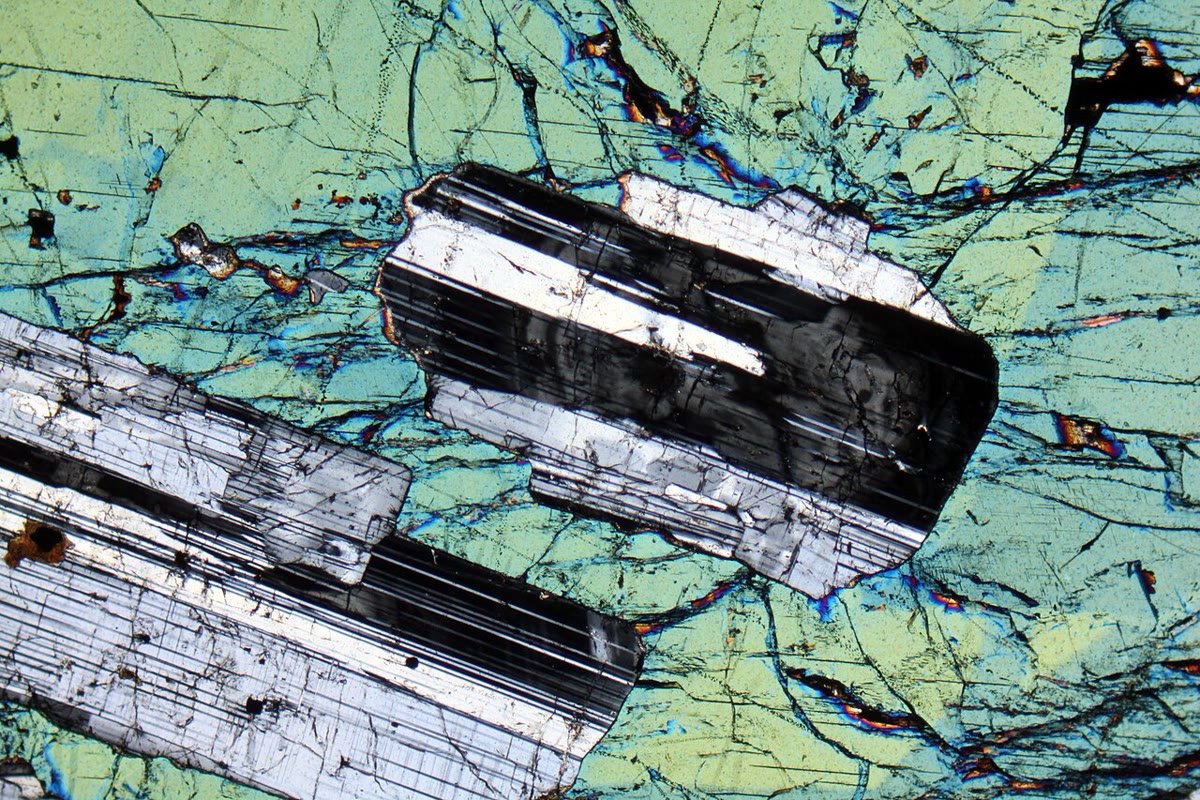
\includegraphics[height=4.6cm]{images/book4/b2-31-ophitic.jpg}\quad
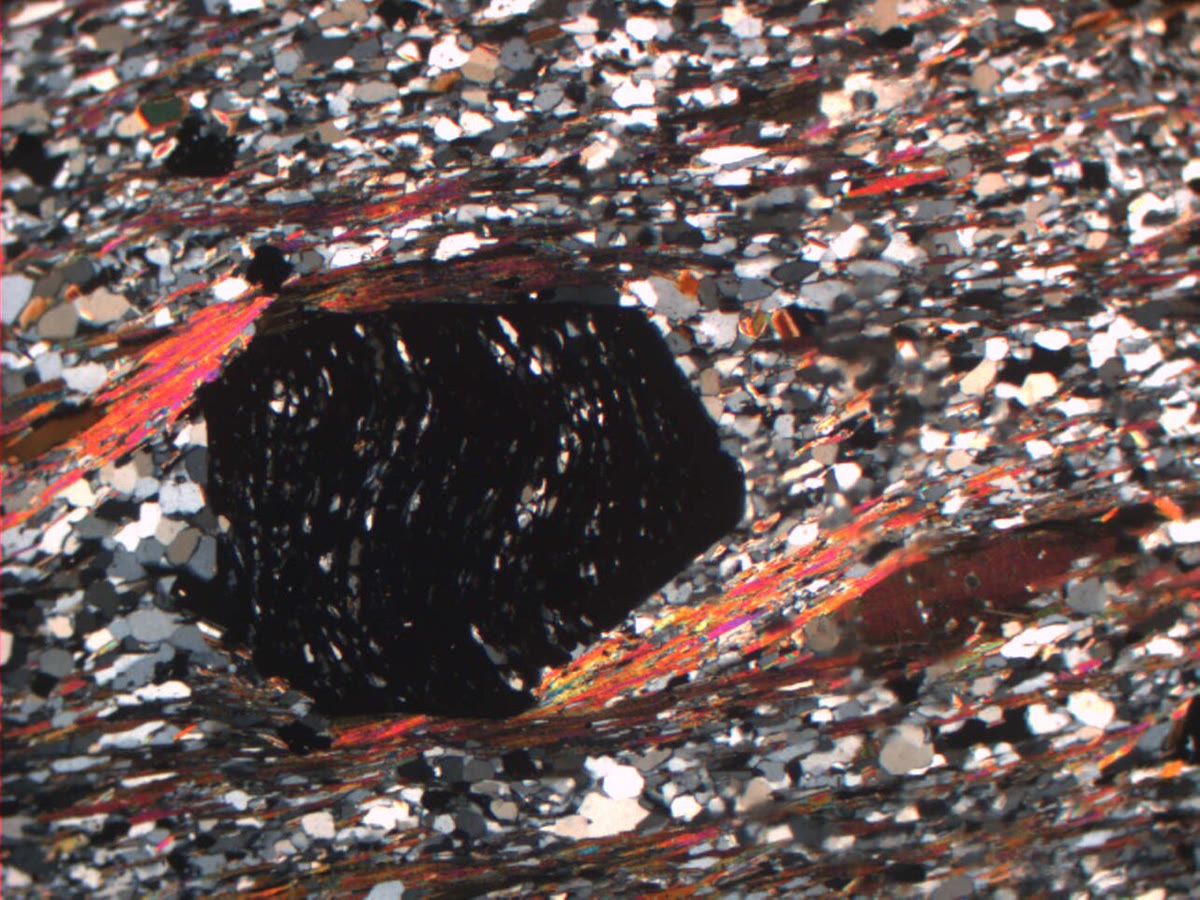
\includegraphics[height=4.6cm]{images/book4/b2-31-garnet-porphyroblast.jpg}
\par\smallskip{\small Two textures between crossed polars. Left: a single crystal of augite (blue
and green) encloses laths of plagioclase striped by their twinning, the arrangement of an \omterm{def:b2:field-lab-methods-2:textures}{ophitic
texture}; field of view \qty{7}{mm}. Photograph Strekeisen, CC BY-SA 4.0 (Wikimedia Commons).
Right: a garnet--mica schist. The garnet, black because it is isotropic, is a large crystal that
grew in the solid state; inclusions of quartz cross it in trails, and the foliation of muscovite
(bright colours), biotite (brown) and quartz (grey) bends around it. Photograph Jackdann88,
CC BY 3.0 (Wikimedia Commons).}
\end{omfigure}
% ledger: photo:b2-31-ophitic, photo:b2-31-garnet

Metamorphic minerals do not all grow at the same pace. Some species overgrow the others into very large crystals,
which engulf the small grains around them as they grow.

\begin{definition}[Porphyroblast, poikiloblast, inclusion trail, corona]\label{def:b2:field-lab-methods-2:porphyroblast}
A \emph{porphyroblast}\index{porphyroblast} is a large crystal that grew during \omterm{def:b2:metamorphic-facies:metamorphism}{metamorphism}
within a finer-grained groundmass; garnet, staurolite, cordierite and chloritoid form them, from
millimetres to several centimetres across. A \emph{poikiloblast}\index{poikiloblast} is a
porphyroblast that contains many inclusions of other minerals. An \emph{inclusion
trail}\index{inclusion trail} is a line of aligned inclusions inside a porphyroblast, which
preserves the fabric of the groundmass at the time the crystal overgrew it. A
\emph{corona}\index{corona (reaction texture)} is a rim of one or more new minerals completely
surrounding a mineral that was breaking down, because it had ceased to be stable with its
neighbours: a reaction texture, frozen before the reaction was complete.
\end{definition}
% ledger: bgsM:textures, ouVM:textures

Comparing the \omterm{def:b2:field-lab-methods-2:porphyroblast}{inclusion trail} ($S_i$, the internal fabric) with the foliation outside the crystal
($S_e$, the external fabric) dates the growth of a \omterm{def:b2:field-lab-methods-2:porphyroblast}{porphyroblast} relative to the deformation that
made the foliation. The criteria below, drawn in the figure, are those of standard teaching notes.
% ledger: ucsbH:inclusion-trails

\begin{method}[Timing a porphyroblast from its inclusion trails]\label{met:b2:field-lab-methods-2:timing}
Find a section cut perpendicular to the foliation, then compare $S_i$ and $S_e$.
\begin{enumerate}
  \item \textbf{Random inclusions}, $S_e$ deflected around the crystal: it grew before the
        foliation formed (\emph{pre-tectonic}).
  \item \textbf{Straight $S_i$ cut off at the rim}, discontinuous with a deflected $S_e$: it grew
        over an older foliation, between two deformations (\emph{inter-tectonic}).
  \item \textbf{Curved $S_i$}, continuous with $S_e$: it grew while the foliation formed, rotating
        or being overgrown as it grew (\emph{syn-tectonic}; the spiral of a snowball garnet).
  \item \textbf{Straight $S_i$ continuous with an undeflected $S_e$}: it grew after the foliation
        (\emph{post-tectonic}).
\end{enumerate}
\end{method}

\begin{omfigure}
\centering
\begin{tikzpicture}[x=1cm, y=1cm, font=\scriptsize]
% schematic after the criteria of ledger ucsbH:inclusion-trails
% panel 1: pre-tectonic
\begin{scope}[shift={(0,0)}]
\draw[omExo, line width=0.5pt] (-1.5,0.95) .. controls (-0.6,0.95) and (-0.5,0.85) .. (0,0.85) .. controls (0.5,0.85) and (0.6,0.95) .. (1.5,0.95);
\draw[omExo, line width=0.5pt] (-1.5,-0.95) .. controls (-0.6,-0.95) and (-0.5,-0.85) .. (0,-0.85) .. controls (0.5,-0.85) and (0.6,-0.95) .. (1.5,-0.95);
\draw[omExo, line width=0.5pt] (-1.5,0.45) .. controls (-0.9,0.45) and (-0.85,0.78) .. (0,0.78) .. controls (0.85,0.78) and (0.9,0.45) .. (1.5,0.45);
\draw[omExo, line width=0.5pt] (-1.5,-0.45) .. controls (-0.9,-0.45) and (-0.85,-0.78) .. (0,-0.78) .. controls (0.85,-0.78) and (0.9,-0.45) .. (1.5,-0.45);
\draw[omExo, line width=0.5pt] (-1.5,0) -- (-0.78,0); \draw[omExo, line width=0.5pt] (0.78,0) -- (1.5,0);
\filldraw[fill=omThm!15, draw=omThm, line width=0.6pt] (0,0) circle (0.72);
\draw[black, line width=0.7pt] (-0.4,0.2) -- (-0.25,0.35); \draw[black, line width=0.7pt] (0.1,0.35) -- (0.3,0.2);
\draw[black, line width=0.7pt] (-0.35,-0.2) -- (-0.15,-0.25); \draw[black, line width=0.7pt] (0.2,-0.15) -- (0.25,-0.4);
\draw[black, line width=0.7pt] (-0.05,0.05) -- (0.05,-0.1); \draw[black, line width=0.7pt] (0.35,0.0) -- (0.5,0.12);
\node at (0,-1.3) {pre-tectonic};
\end{scope}
% panel 2: inter-tectonic
\begin{scope}[shift={(3.4,0)}]
\draw[omExo, line width=0.5pt] (-1.5,0.95) .. controls (-0.6,0.95) and (-0.5,0.85) .. (0,0.85) .. controls (0.5,0.85) and (0.6,0.95) .. (1.5,0.95);
\draw[omExo, line width=0.5pt] (-1.5,-0.95) .. controls (-0.6,-0.95) and (-0.5,-0.85) .. (0,-0.85) .. controls (0.5,-0.85) and (0.6,-0.95) .. (1.5,-0.95);
\draw[omExo, line width=0.5pt] (-1.5,0.45) .. controls (-0.9,0.45) and (-0.85,0.78) .. (0,0.78) .. controls (0.85,0.78) and (0.9,0.45) .. (1.5,0.45);
\draw[omExo, line width=0.5pt] (-1.5,-0.45) .. controls (-0.9,-0.45) and (-0.85,-0.78) .. (0,-0.78) .. controls (0.85,-0.78) and (0.9,-0.45) .. (1.5,-0.45);
\draw[omExo, line width=0.5pt] (-1.5,0) -- (-0.78,0); \draw[omExo, line width=0.5pt] (0.78,0) -- (1.5,0);
\filldraw[fill=omThm!15, draw=omThm, line width=0.6pt] (0,0) circle (0.72);
\begin{scope}
\clip (0,0) circle (0.66);
\foreach \k in {-0.6,-0.3,0,0.3,0.6} {\draw[black, line width=0.7pt, dash pattern=on 2pt off 1.5pt] (-0.8,\k-0.45) -- (0.8,\k+0.45);}
\end{scope}
\node at (0,-1.3) {inter-tectonic};
\end{scope}
% panel 3: syn-tectonic
\begin{scope}[shift={(6.8,0)}]
\draw[omExo, line width=0.5pt] (-1.5,0.8) -- (1.5,0.8);
\draw[omExo, line width=0.5pt] (-1.5,-0.8) -- (1.5,-0.8);
\draw[omExo, line width=0.5pt] (-1.5,0.4) -- (-0.6,0.4); \draw[omExo, line width=0.5pt] (0.6,0.4) -- (1.5,0.4);
\draw[omExo, line width=0.5pt] (-1.5,0) -- (-0.72,0); \draw[omExo, line width=0.5pt] (0.72,0) -- (1.5,0);
\draw[omExo, line width=0.5pt] (-1.5,-0.4) -- (-0.6,-0.4); \draw[omExo, line width=0.5pt] (0.6,-0.4) -- (1.5,-0.4);
\filldraw[fill=omThm!15, draw=omThm, line width=0.6pt] (0,0) circle (0.72);
\draw[black, line width=0.7pt, dash pattern=on 2pt off 1.5pt] (-0.6,0.4) .. controls (-0.35,0.4) and (-0.2,0.3) .. (-0.05,0.4) .. controls (0.1,0.5) and (0.35,0.4) .. (0.6,0.4);
\draw[black, line width=0.7pt, dash pattern=on 2pt off 1.5pt] (-0.72,0) .. controls (-0.3,0) and (-0.3,-0.45) .. (0,0) .. controls (0.3,0.45) and (0.3,0) .. (0.72,0);
\draw[black, line width=0.7pt, dash pattern=on 2pt off 1.5pt] (-0.6,-0.4) .. controls (-0.35,-0.4) and (-0.1,-0.5) .. (0.05,-0.4) .. controls (0.2,-0.3) and (0.35,-0.4) .. (0.6,-0.4);
\node at (0,-1.3) {syn-tectonic};
\end{scope}
% panel 4: post-tectonic
\begin{scope}[shift={(10.2,0)}]
\foreach \k in {-0.8,-0.4,0,0.4,0.8} {\draw[omExo, line width=0.5pt] (-1.5,\k) -- (1.5,\k);}
\filldraw[fill=omThm!15, draw=omThm, line width=0.6pt] (0,0) circle (0.72);
\begin{scope}
\clip (0,0) circle (0.66);
\foreach \k in {-0.8,-0.4,0,0.4,0.8} {\draw[black, line width=0.7pt, dash pattern=on 2pt off 1.5pt] (-0.8,\k) -- (0.8,\k);}
\end{scope}
\node at (0,-1.3) {post-tectonic};
\end{scope}
\end{tikzpicture}
\par\smallskip{\small \omterm{def:b2:field-lab-methods-2:porphyroblast}{Inclusion trails} (black, dashed) in a \omterm{def:b2:field-lab-methods-2:porphyroblast}{porphyroblast} (red) and the foliation
outside it (grey), in sections perpendicular to the foliation (schematic). From left to right:
inclusions grown before the foliation, which bends around the crystal; a straight older fabric cut
off at the rim; a trail that curves into the foliation, the crystal having rotated as it grew; a
straight trail that continues the undisturbed foliation.}
\end{omfigure}

Petrography is also quantitative. The proportions of the minerals of a coarse-grained igneous rock
name it on the \omterm{def:b2:magmatic-series:qapf}{QAPF diagram} (\cref{ch:b2:magmatic-series}), and they are measured under the
microscope.

\begin{definition}[Modal analysis, point counting]\label{def:b2:field-lab-methods-2:modal}
A \emph{modal analysis}\index{modal analysis} is the measurement of the \omterm{def:b2:magmatic-series:qapf}{modal composition} of a
rock. In \emph{point counting}\index{point counting}, a thin
section is moved under the cross-wires of the microscope in equal steps along a regular grid, and
the mineral under the cross-wires is recorded at each point; the proportion of the points that
fall on a mineral estimates its proportion in the rock.
\end{definition}

\begin{proposition}[What point counting measures, and how well]\label{prop:b2:field-lab-methods-2:counting}
(a) In a rock without preferred orientation, the area fraction of a mineral in a section placed
at random has, on average, the value of its volume fraction. (b) If $n$ points fall independently
on a mineral of area fraction $p$, the counted proportion $\hat p = k/n$ has mean $p$ and standard
deviation
\begin{equation}
\sigma = \sqrt{\frac{p(1-p)}{n}} , \qquad\text{so that}\qquad n = \frac{p(1-p)}{\sigma^2}
\label{eq:b2:field-lab-methods-2:binomial}
\end{equation}
points are needed to reach a standard deviation $\sigma$.
\end{proposition}

\begin{proof}
(a) Cut a block of rock of height $H$ into parallel sections of area $S$. The volume of the
mineral is $\int_0^H a(z)\,\mathrm{d}z$, where $a(z)$ is its area in the section at height $z$;
dividing by the volume $SH$, the volume fraction is the mean of the area fraction $a(z)/S$ over
all heights, which is the expected value for a height drawn at random. (b) Each point falls on the
mineral with probability $p$, independently of the others, so the number $k$ of hits follows the
binomial distribution of parameters $n$ and $p$, of mean $np$ and variance $np(1-p)$. Dividing by
$n$ gives the mean $p$ and the variance $p(1-p)/n$ of $\hat p$.
\end{proof}

The proof of (b) supposes independent points, which a grid step larger than the grains
approaches. For a mineral making \qty{30}{\percent} of a rock, 500 points give $\sigma =
\sqrt{0.3 \times 0.7/500} = 0.020$, two percentage points; reaching one percentage point needs
$0.21/0.01^2 = 2100$ points, four times as many, because $\sigma$ falls only as $1/\sqrt n$. The
relative error, $\sigma/p = \sqrt{(1-p)/(np)}$, is worst for the rare minerals (figure below,
left). The counted proportions are then recalculated to name the rock: a mode with
\qty{10}{\percent} quartz, 30 alkali feldspar, 20 plagioclase and 40 mafic minerals gives Q, A and
P of 16.7, 50.0 and 33.3 once the three felsic components are brought to a sum of 100. On the QAP
triangle a rock with Q between 20 and 60 is a granite when its ratio P/(A+P) lies between 10 and
\qty{65}{\percent}: a syenogranite below 35, a monzogranite above; from 65 to 90 it is a
granodiorite, above 90 a tonalite. The colour index $M'$ is the proportion of dark minerals, that
is the mafic and related minerals other than muscovite, apatite and primary carbonate; a rock is
leucocratic below 35, mesocratic from 35 to 65, melanocratic from 65 to 90.
% ledger: bgsI:qapf, bgsI:colour-index

\begin{omfigure}
\centering
\begin{minipage}[b]{0.49\linewidth}\centering
\begin{tikzpicture}
\begin{axis}[omrecord, width=0.96\linewidth, height=5.0cm, xmode=log, xmin=100, xmax=3000,
  ymin=0, ymax=45, xlabel={points counted, $n$}, ylabel={relative error $\sigma/p$ (\unit{\percent})},
  xtick={100,300,1000,3000}, xticklabels={100,300,1000,3000}, log ticks with fixed point,
  tick label style={font=\scriptsize}, label style={font=\small}]
% computed in figdata/bachelor-2/labmethods.py part pc (binomial counting)
\addplot[omThm, line width=1.1pt] table[x=n, y=rel05] {figdata/out/bachelor-2-labmethods-pc.dat};
\addplot[omProp, line width=1.1pt] table[x=n, y=rel20] {figdata/out/bachelor-2-labmethods-pc.dat};
\addplot[omDef, line width=1.1pt] table[x=n, y=rel50] {figdata/out/bachelor-2-labmethods-pc.dat};
\node[font=\scriptsize, text=omThm, anchor=south west] at (axis cs:330,24) {$p = 0.05$};
\node[font=\scriptsize, text=omProp, anchor=south west] at (axis cs:104,21.5) {$p = 0.2$};
\node[font=\scriptsize, text=omDef, anchor=south west] at (axis cs:104,10.3) {$p = 0.5$};
\end{axis}
\end{tikzpicture}
\end{minipage}\hfill
\begin{minipage}[b]{0.49\linewidth}\centering
\begin{tikzpicture}
\begin{axis}[omrecord, width=0.96\linewidth, height=5.0cm, xmin=52, xmax=76, ymin=-1.0, ymax=0.75,
  xlabel={recommended \ce{SiO2} (\unit{\percent})}, ylabel={difference (\unit{\percent})},
  tick label style={font=\scriptsize}, label style={font=\small},
  ytick={-0.8,-0.4,0,0.4}, yticklabel style={/pgf/number format/fixed}]
% data: figdata/bachelor-2/labmethods.py part xrf; ledger: usgsT:sio2-table
\addplot[black!40, densely dotted] coordinates {(52,0) (76,0)};
\addplot[only marks, mark=*, mark size=1.5pt, omDef, error bars/.cd, y dir=both, y explicit]
  table[x=rec, y=diff, y error=s] {figdata/out/bachelor-2-labmethods-xrf.dat};
\node[font=\scriptsize, anchor=east] at (axis cs:73.0,-0.62) {RGM-1};
\node[font=\scriptsize, anchor=west] at (axis cs:56.6,0.40) {JA-2};
\node[font=\scriptsize, anchor=west] at (axis cs:60.8,-0.55) {AMH-1};
\node[font=\scriptsize, anchor=north] at (axis cs:54.1,-0.10) {BCR-2};
\end{axis}
\end{tikzpicture}
\end{minipage}
\par\smallskip{\small Left: relative standard error of a modal proportion $p$ measured by \omterm{def:b2:field-lab-methods-2:modal}{point
counting}, \eqref{eq:b2:field-lab-methods-2:binomial}, for a rare, a common and an abundant mineral.
Right: accuracy of silica by X-ray fluorescence on \omterm{def:b2:field-lab-methods-2:xrf}{fused beads} for ten rock reference materials,
from basalt to granite; each dot is the mean of 2 to 30 analyses minus the recommended value, with
the standard deviation of the analyses as a bar. Data: Taggart and Siems (2002), USGS.}
\end{omfigure}
% ledger: usgsT:sio2-table

\section{Whole-rock analysis}\label{sec:b2:field-lab-methods-2:whole-rock}

A whole-rock analysis needs a sample that represents the rock: a teaching sheet of the SERC
geochemistry collection advises collecting a sample several times larger than the largest grain,
which is crushed in stages and ground to a fine powder. The workhorse for the major elements is
X-ray fluorescence. An X-ray beam, typically from a tube with a rhodium target, ejects inner
electrons from the atoms of the sample, and each element then emits X-rays at its own
characteristic energies (Moseley's law, from the physics books).
% ledger: sercX:xrf-scope

\begin{definition}[X-ray fluorescence analysis, fused bead, loss on ignition]\label{def:b2:field-lab-methods-2:xrf}
\emph{X-ray fluorescence analysis}\index{X-ray fluorescence analysis} measures the concentrations
of the elements of a solid from the intensities of the characteristic X-rays it emits under an
X-ray beam, by comparison with standards of known composition. A \emph{fused
bead}\index{fused bead} is a glass disc made by melting a weighed rock powder with a weighed flux,
such as lithium tetraborate, and casting the melt; it is homogeneous whatever the grains of the
powder were. The \emph{loss on ignition}\index{loss on ignition} is the fraction of its mass that
a powder loses when heated at a fixed high temperature, mostly water and carbon dioxide driven off.
\end{definition}
% ledger: sercX:xrf-scope, usgsT:procedure

The intensity of a line is proportional to the abundance of its element only when the samples and
the standards are alike, since the other elements absorb and enhance the radiation: these matrix
effects, and those of grain size, are why the powder is melted into a glass, and why a mathematical
correction is still applied. XRF measures the ten major elements and, above about \qty{1}{ppm},
\omterm{def:b2:elements-in-the-earth:trace}{trace elements} such as Rb, Sr, Zr and Ba, with detection limits of a few parts per million. It is
weak for the light elements (atomic number below 11) and sees neither isotopes nor the oxidation
state of iron.
% ledger: sercX:xrf-scope, usgsT:procedure

\begin{inthelab}[A batch of fused beads]
In a procedure published by the US Geological Survey, \qty{0.8000}{g} of rock powder is heated in a
platinum--gold crucible at \qty{925}{\celsius} for 40 minutes, and the loss of mass is reported as
the \omterm{def:b2:field-lab-methods-2:xrf}{loss on ignition}. Lithium tetraborate is added, enough to leave \qty{8.0000}{g} after fusion;
seven crucibles at a time are held in a furnace at \qty{1120}{\celsius} and rocked for 35 minutes,
then poured into moulds. In the spectrometer, an end-window rhodium tube irradiates each bead, and
the intensities of the ten major elements are compared with those of standards. An analysis whose
oxides add up to less than 97 or more than \qty{101}{\percent} is repeated; one analyst completes
about 250 samples a month.
\end{inthelab}
% ledger: usgsT:procedure

The standards are themselves rocks, analysed so often that their composition is known better than
any single analysis can measure it.

\begin{definition}[Geochemical reference material]\label{def:b2:field-lab-methods-2:rm}
A \emph{geochemical reference material}\index{geochemical reference material} is a natural rock,
mineral or sediment, ground and homogenised in a large batch, for which one or more concentrations
have well-established or certified values, used to calibrate instruments and to test the accuracy
of a method.
\end{definition}
% ledger: usgsOFR:rm

The USGS basalt BHVO-2, collected in 1995 from a lava that overflowed from the Halemaumau crater of
Kilauea in 1919, has a recommended \ce{SiO2} of \qty{49.60}{\percent} and \qty{394.1}{ppm} of
strontium. A laboratory checks its own trueness by running such materials as unknowns, at the low,
middle and high ends of its range: in the figure above, the USGS method recovers silica within
\qty{0.6}{\percent} of the recommended value for all ten rocks, from \ce{SiO2} 54 to
\qty{74}{\percent}. Its blanks fix its limits: the limit of detection is taken as three standard
deviations of independently prepared blanks, the lower reporting limit as five, and ten are often
suggested for the limit of quantification.
% ledger: usgs:bhvo2-origin, usgs:bhvo2-major, usgs:bhvo2-trace, usgsOFR:rm, usgsOFR:lod, usgsT:sio2-table

\begin{method}[Calibrating and checking a whole-rock analysis]\label{met:b2:field-lab-methods-2:calibration}
\begin{enumerate}
  \item \textbf{Calibrate.} Measure the intensity $I$ of each element in beads of several reference
        materials, and fit the least-squares line $c = aI + b$ of the recommended concentration
        against the intensity.
  \item \textbf{Measure.} Convert the intensity of each unknown into a concentration with the line.
  \item \textbf{Check.} Run a reference material as an unknown in every batch and compare it with
        its recommended value; add the oxides and the \omterm{def:b2:field-lab-methods-2:xrf}{loss on ignition}, which should come close
        to \qty{100}{\percent}.
  \item \textbf{Report.} Give the analysis as measured with its \omterm{def:b2:field-lab-methods-2:xrf}{loss on ignition}; for the
        classification diagrams, recalculate the oxides to a sum of 100 without the volatiles.
\end{enumerate}
\end{method}

\section{Mineral analysis: the electron microprobe}\label{sec:b2:field-lab-methods-2:microprobe}

XRF gives the composition of the whole rock. The zoning of a garnet \omterm{def:b2:field-lab-methods-2:porphyroblast}{porphyroblast}, the reactions
recorded by a \omterm{def:b2:field-lab-methods-2:porphyroblast}{corona} or the mineral pairs of a \omterm{def:b2:pt-paths:thermobarometry}{geothermometer} need the composition of a single
grain, and of points within it.

\begin{definition}[Electron microprobe, wavelength-dispersive spectrometry]\label{def:b2:field-lab-methods-2:epma}
An \emph{electron microprobe}\index{electron microprobe} is an instrument that focuses a beam of
electrons on a spot of a polished section and measures the characteristic X-rays emitted there,
giving a quantitative analysis of a volume a few micrometres across. In
\emph{wavelength-dispersive spectrometry}\index{wavelength-dispersive spectrometry}, the X-rays fall
on an analytical crystal that reflects to a detector only the wavelength satisfying Bragg's law at
its angle; crystal and detector move together on a circle (the Rowland circle) to select each
element's line in turn.
\end{definition}
% ledger: sercE:epma-spot, sercW:wds

Spots can be as small as 1 to \qty{2}{\micro\metre}, and detection reaches a few tens of ppm by
weight, for elements from boron (atomic number 5) upward. The counts are compared with those of
standards and corrected for the effects of atomic number, absorption and fluorescence (a ZAF
correction). A probe with four or five crystal spectrometers measures 10 to 12 elements in one
analysis. It cannot detect hydrogen, helium or lithium, so the water of micas and amphiboles is
missing from their totals; it cannot tell ferrous from ferric iron; and it reports oxides, from
which the mineral formula is recalculated as in the Year 1 volume.
% ledger: sercE:epma-spot, sercE:epma-limits, sercW:wds

\begin{inthelab}[A day on the microprobe]
\begin{minipage}[t]{0.55\linewidth}\vspace{0pt}
Thin sections for the microprobe are usually rectangles of \qtyproduct{27 x 46}{mm}, ground to
\qty{30}{\micro\metre} and left without a cover glass, then polished flat. Most silicates are
electrical insulators, so the section is coated with a thin conducting film, most commonly carbon,
to carry away the charge of the beam. The analyst marks the grains to measure on photographs taken
under the polarising microscope, loads the standards with the sections, and lets the instrument run
through a list of points: a traverse from core to rim across a garnet, say.
\end{minipage}\hfill
\begin{minipage}[t]{0.42\linewidth}\vspace{0pt}
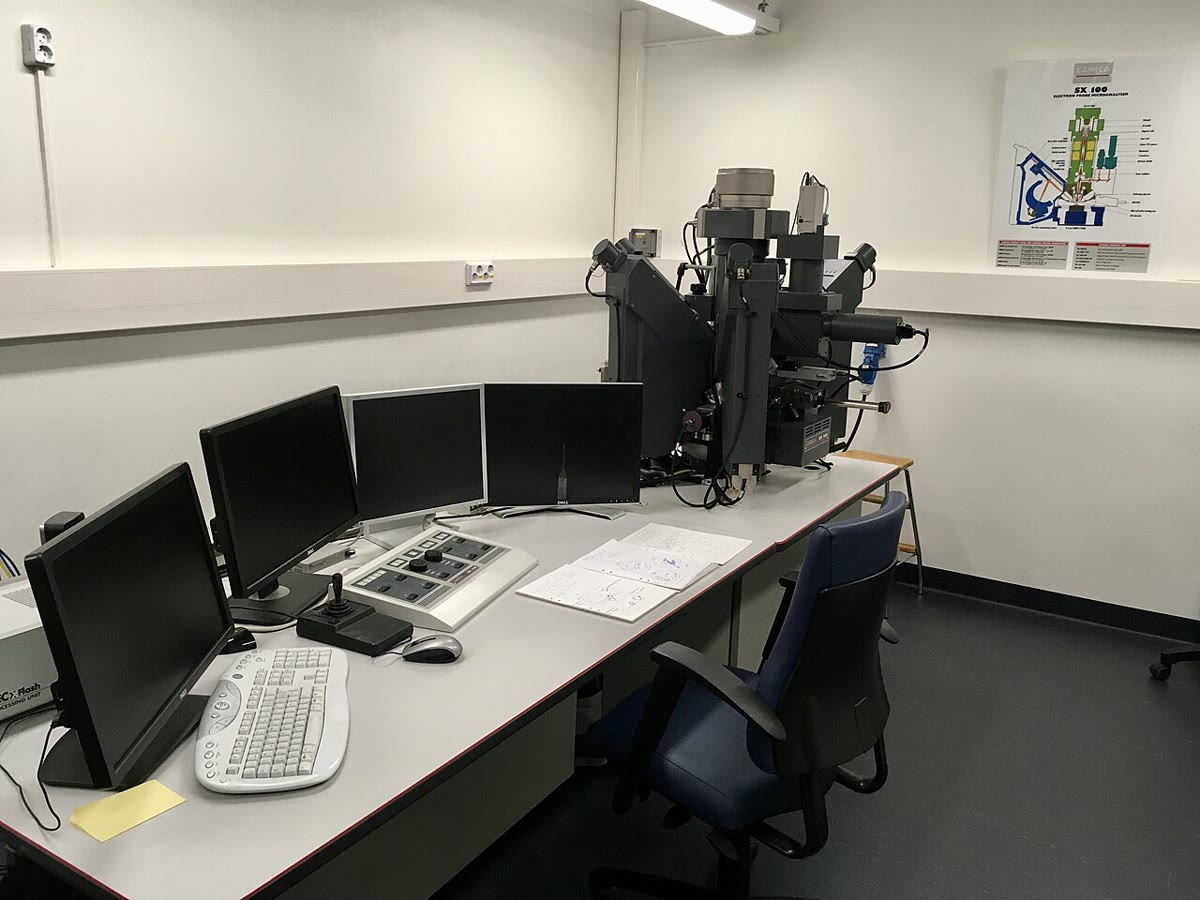
\includegraphics[width=\linewidth]{images/book4/b2-31-microprobe.jpg}
\par\smallskip{\scriptsize An \omterm{def:b2:field-lab-methods-2:epma}{electron microprobe}: the electron column, with its spectrometers
around it, and the operator's desk. Photograph Kallerna, CC BY-SA 4.0 (Wikimedia Commons).}
\end{minipage}
\end{inthelab}
% ledger: sercE:epma-spot, sercE:coating, photo:b2-31-microprobe

\section{Isotope analysis}\label{sec:b2:field-lab-methods-2:isotopes}

\omterm{def:b2:isotope-geochemistry:tracer}{Radiogenic isotope tracers} and ages (\cref{ch:b2:isotope-geochemistry}) rest on ratios measured
to 0.01--\qty{0.001}{\percent}, on elements separated from the rock by dissolution
and ion-exchange chromatography in a clean laboratory, with filtered air (typically Class 100 to
1000) so that dust adds nothing to the small amounts analysed.
% ledger: sercT:tims

\begin{definition}[Thermal ionisation mass spectrometry, multi-collector ICP-MS, mass bias]\label{def:b2:field-lab-methods-2:tims}
In \emph{thermal ionisation mass spectrometry}\index{thermal ionisation mass spectrometry} (TIMS), a
purified element is loaded on a thin metal ribbon and ionised by heating it under vacuum; the ions
are accelerated across a potential of up to \qty{10}{kV}, separated by mass in a magnetic sector
and collected. In \emph{multi-collector ICP-MS}\index{multi-collector ICP-MS} the ions come from an
inductively coupled plasma, which ionises elements that are hard to ionise thermally, and several
collectors measure the beams of different masses at the same time. The \emph{mass
bias}\index{mass bias} of a measurement is the departure of a measured isotope ratio from the true
ratio of the sample caused by the instrument, which transmits or ionises one mass more readily than
another.
\end{definition}
% ledger: sercT:tims, sercM:mcicpms

Both instruments reach this precision. TIMS ionises generally less than
\qty{1}{\percent} of the atoms, and its \omterm{def:b2:field-lab-methods-2:tims}{mass bias} changes continually during a run. The bias is corrected by fixing the ratio of two isotopes that no
decay changes, which requires an element with at least three isotopes, two of them stable and not
radiogenic. For strontium, $^{86}\mathrm{Sr}/^{88}\mathrm{Sr}$ is fixed at 0.1194, and one common
form of the correction is the exponential law.
% ledger: sercT:tims, sercM:mcicpms, cheong14:mass-bias, ciaaw:sr-isotopes

\begin{proposition}[Exponential law of mass bias]\label{prop:b2:field-lab-methods-2:bias}
Suppose that every measured ratio of two isotopes of masses $m_i$ and $m_j$ is related to the true
ratio by $R_{ij}^{\mathrm{true}} = R_{ij}^{\mathrm{meas}}\,(m_i/m_j)^{\beta}$, with one exponent
$\beta$ for the whole run. Then the measured ratio $r$ of a reference pair, whose true value
$r_0$ is known, gives
\begin{equation}
\beta = \frac{\ln(r_0/r)}{\ln(m_k/m_l)}
\label{eq:b2:field-lab-methods-2:beta}
\end{equation}
for the reference pair $k/l$, and every other ratio is corrected with the same $\beta$.
\end{proposition}

\begin{proof}
Applied to the reference pair, the law reads $r_0 = r\,(m_k/m_l)^\beta$; taking logarithms,
$\ln(r_0/r) = \beta\ln(m_k/m_l)$, which is \eqref{eq:b2:field-lab-methods-2:beta}. The exponent is
common to all the ratios of the run by hypothesis, so it corrects each of them.
\end{proof}

For strontium the reference pair is $^{86}\mathrm{Sr}/^{88}\mathrm{Sr}$ with $r_0 = 0.1194$, and
the corrected $^{87}\mathrm{Sr}/^{86}\mathrm{Sr}$ is the measured ratio times
$(m_{87}/m_{86})^\beta$. The CIAAW abundances, \qty{9.86}{\percent} of strontium-86 and
\qty{82.58}{\percent} of strontium-88, give the same value. Every session also runs an \omterm{def:b2:isotope-geochemistry:standards}{isotope
reference standard}: one laboratory measured $^{87}\mathrm{Sr}/^{86}\mathrm{Sr} = 0.710252 \pm
0.000007$ on the reference material NBS~987 in seven runs.
% ledger: cheong14:mass-bias, ciaaw:sr-isotopes

Ratios alone do not give a concentration. For that, a known amount of a \emph{spike}, a solution of
the element artificially enriched in one isotope, is mixed with the dissolved sample before the
chemistry, and the ratio is measured in the mixture. The TIMS laboratories use it for both
concentrations and parent-to-daughter ratios.
% ledger: sercT:tims

\begin{proposition}[Isotope dilution]\label{prop:b2:field-lab-methods-2:id}
Let a sample contain $N_x$ moles of a reference isotope $b$ and a spike $N_s$ moles of it, and let
$R_x$, $R_s$ and $R_m$ be the ratios of a second isotope $a$ to $b$ in the sample, the spike and
the mixture. Then
\begin{equation}
N_x = N_s\,\frac{R_s - R_m}{R_m - R_x} .
\label{eq:b2:field-lab-methods-2:id}
\end{equation}
A relative error $\varepsilon$ on $R_m$ gives $N_x$ the relative error $\mathcal{M}\varepsilon$,
with the error magnification
\begin{equation}
\mathcal{M} = \frac{R_m\,(R_s - R_x)}{(R_s - R_m)(R_m - R_x)} ,
\label{eq:b2:field-lab-methods-2:mag}
\end{equation}
which is smallest when $R_m = \sqrt{R_s R_x}$.
\end{proposition}
\index{isotope dilution}

\begin{proof}
Isotope $a$ is conserved on mixing: $R_m(N_x + N_s) = R_x N_x + R_s N_s$, so $N_x(R_m - R_x) =
N_s(R_s - R_m)$, which is \eqref{eq:b2:field-lab-methods-2:id}. Its logarithmic derivative is
$\mathrm{d}\ln N_x/\mathrm{d}\ln R_m = R_m\,[-1/(R_s - R_m) - 1/(R_m - R_x)] = -\mathcal{M}$, with
$\mathcal{M}$ as in \eqref{eq:b2:field-lab-methods-2:mag}. Up to the positive constant $R_s - R_x$,
$1/\mathcal{M} = (R_s - R_m)(R_m - R_x)/R_m = R_s + R_x - R_m - R_sR_x/R_m$, whose derivative
$-1 + R_sR_x/R_m^2$ vanishes at $R_m = \sqrt{R_sR_x}$, a maximum of $1/\mathcal{M}$.
\end{proof}

\omterm{prop:b2:field-lab-methods-2:id}{Isotope dilution} needs neither a calibration line nor a complete recovery of the element through
the chemistry: once spike and sample are mixed, losses take both alike. A published strontium
spike, for instance, contains \qty{99.65}{\percent} strontium-84, with
$^{84}\mathrm{Sr}/^{88}\mathrm{Sr} = 561.4$ and $^{86}\mathrm{Sr}/^{88}\mathrm{Sr} = 0.7661$, at
\qty{15.271}{\micro\gram} of strontium per gram of solution. Its 86/88 ratio shows why the \omterm{def:b2:field-lab-methods-2:tims}{mass
bias} of a spiked mixture cannot be corrected by fixing $^{86}\mathrm{Sr}/^{88}\mathrm{Sr}$ at its
natural value: the spike has moved that ratio.
% ledger: cheong14:spike, cheong14:mass-bias

\section{A mapping campaign on the Varden inlier}\label{sec:b2:field-lab-methods-2:campaign}

In the core of the Varden anticline, erosion has cut through the sandstone cover and exposed the
basement: schist intruded by a granite. A campaign that is to supply the laboratory begins in the
field. Two traverses are walked west to east across the inlier, with a station every
\qty{100}{m}; at each the unit is recorded, and fresh samples are taken where the rock is
unweathered, numbered with the station, and, where fabrics are to be measured, oriented. The figure
shows what the stations meet: of the 30, ten are on granite, ten on the sandstone cover, one on
the schist, one on limestone and eight on the alluvium of the valley floor, where no rock crops
out.

\begin{omfigure}
\centering
\begin{tikzpicture}
\begin{axis}[axis equal image, xmin=2.4, xmax=4.6, ymin=3.1, ymax=5.0, width=0.66\linewidth,
  tick label style={font=\scriptsize}, xlabel={east (km)}, ylabel={north (km)},
  label style={font=\small}]
% units: figdata/shared/region.py (read only); stations: figdata/bachelor-2/labmethods.py part stations
\addplot[lith schist, draw=black, line width=0.3pt, even odd rule] table {figdata/out/shared-region-unit-schist.dat};
\addplot[lith granite, draw=black, line width=0.3pt, even odd rule] table {figdata/out/shared-region-unit-granite.dat};
\addplot[om lith={icsTriassic!35}{om sand}, draw=black, line width=0.3pt, even odd rule] table {figdata/out/shared-region-unit-sandstone.dat};
\addplot[om lith={icsJurassic!40}{om limestone}, draw=black, line width=0.3pt, even odd rule] table {figdata/out/shared-region-unit-limestone.dat};
\addplot[om lith={icsJurassic!15}{om shale}, draw=black, line width=0.3pt, even odd rule] table {figdata/out/shared-region-unit-shale.dat};
\addplot[lith alluvium, draw=black, line width=0.3pt, even odd rule] table {figdata/out/shared-region-unit-alluvium.dat};
\addplot[river] table {figdata/out/shared-region-river.dat};
\addplot[only marks, mark=*, mark size=1.6pt, mark options={fill=white, draw=black}]
  table[x=x_km, y=y_km] {figdata/out/bachelor-2-labmethods-stations.dat};
\addplot[only marks, mark=*, mark size=1.6pt, mark options={fill=omThm, draw=black},
  x filter/.expression={\thisrow{unit}==2 ? x : nan}]
  table[x=x_km, y=y_km] {figdata/out/bachelor-2-labmethods-stations.dat};
\node[font=\scriptsize, fill=white, inner sep=1pt, anchor=east] at (axis cs:2.76,3.7) {1};
\node[font=\scriptsize, fill=white, inner sep=1pt, anchor=west] at (axis cs:4.24,3.7) {15};
\node[font=\scriptsize, fill=white, inner sep=1pt, anchor=east] at (axis cs:2.76,4.4) {16};
\node[font=\scriptsize, fill=white, inner sep=1pt, anchor=west] at (axis cs:4.24,4.4) {30};
\draw[black, line width=0.5pt] (axis cs:3.5,4.44) -- (axis cs:3.5,4.62);
\node[font=\scriptsize, fill=white, inner sep=1pt, anchor=south] at (axis cs:3.5,4.62) {station 23};
\pic at (axis cs:4.45,4.75) {northarrow};
\end{axis}
\end{tikzpicture}
\par\smallskip{\small The basement inlier of the Varden Hills with the 30 stations of two west--east
traverses, \qty{100}{m} apart. Red dots: stations on granite. Pink with crosses: granite; grey: schist; purple: Triassic
sandstone; blue: Jurassic limestone; pale blue: Jurassic shale; cream: alluvium of the river, which
flows east. The
granite sample of the weekend problem comes from station 23.}
\end{omfigure}

\begin{inthefield}[Sampling for the laboratory]
\centering
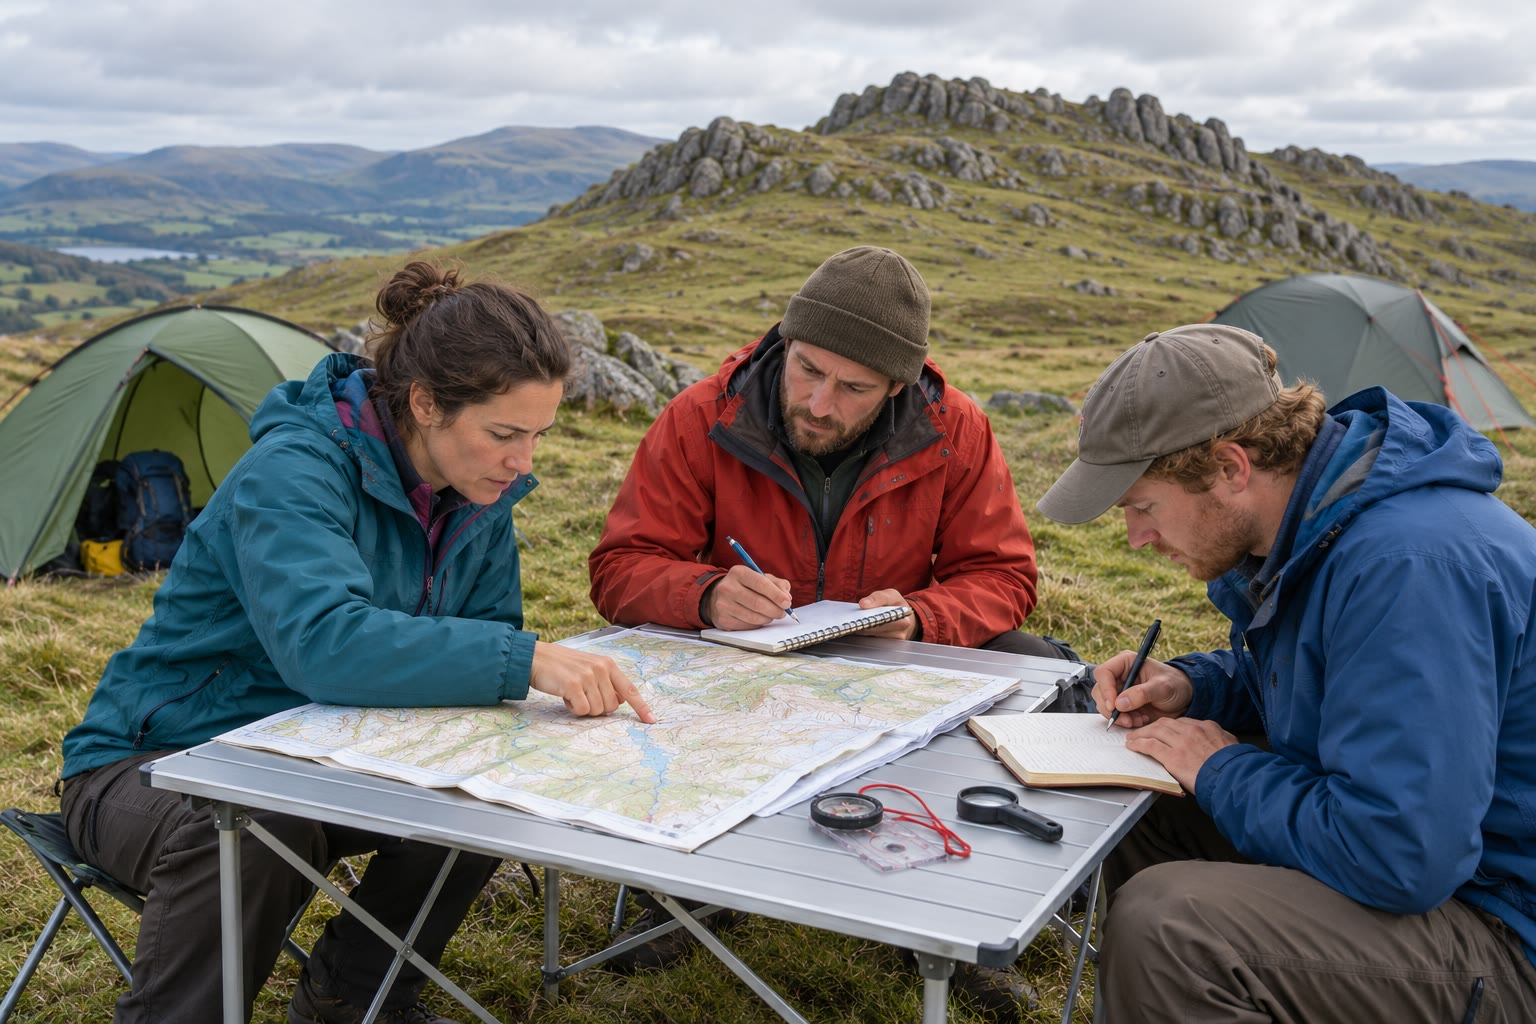
\includegraphics[width=0.56\linewidth]{images/book4/ai/b2-field-camp.jpg}
\par\smallskip{\small A field party plans the next day's traverses (AI-generated illustration).}
\par\medskip\raggedright
In the evening the party transfers the stations to the map, checks that every sample number in the
notebooks matches a bag, and decides which samples go to which laboratory. One sample of each unit
goes to the thin-section laboratory; the freshest granite and schist go
for crushing and whole-rock analysis; a few granite samples are set aside for isotopes. The
station number follows each sample through every step, from the bag to the thin section, the
powder, the bead and the line of a data table, so that any odd result can be traced back to its
outcrop.
\end{inthefield}

\section{The quality of a number}\label{sec:b2:field-lab-methods-2:quality}

Each step of the chain adds its own error, and the methods of this chapter show the two kinds that
the chemistry books distinguish. \omterm{def:b2:field-lab-methods-2:modal}{Point counting} and isotope ratios have mostly random errors, which
shrink as the counts grow, like $1/\sqrt n$; calibration has systematic ones, which repetition does
not reduce and which only a reference material reveals. The figure of the silica analyses shows
both: the bars are the precision of the method, and a dot that misses zero by many times its bar
divided by the square root of the number of analyses is a bias. The same element measured by two
methods, strontium by XRF and by \omterm{prop:b2:field-lab-methods-2:id}{isotope dilution}, is a further check, since the two share no
calibration. Results are reported with their uncertainty, rounded to it, and with the reference
materials run alongside them; a number without them cannot be compared with any other.

\section*{Exercises}\label{sec:b2:field-lab-methods-2:exercises}

Data for the exercises, unless stated otherwise: atomic masses H 1.008, O 15.999, Mg 24.305, Al
26.982, Si 28.085, K 39.098, Sr 87.62; isotope masses $^{86}\mathrm{Sr}$ 85.909261,
$^{87}\mathrm{Sr}$ 86.908878, $^{88}\mathrm{Sr}$ 87.905612; natural strontium
$^{84}\mathrm{Sr}/^{86}\mathrm{Sr} = 0.05680$, \qty{9.86}{\percent} of $^{86}\mathrm{Sr}$; the spike
of the text, $^{84}\mathrm{Sr}/^{86}\mathrm{Sr} = 732.8$, \qty{0.13599}{\percent} of
$^{86}\mathrm{Sr}$, atomic weight 83.9242, \qty{15.271}{\micro\gram\per\gram}. Round to three
significant figures unless stated otherwise.
% ledger: ciaaw:H, ciaaw:O, ciaaw:Mg, ciaaw:Al, ciaaw:Si, ciaaw:K, ciaaw:sr-isotopes, cheong14:spike

\begin{exercise}[$\star$]\label{exo:b2:field-lab-methods-2:1}
(a) Name the texture or the crystal: (i) a dolerite in which plagioclase laths are wholly enclosed in
large augite crystals; (ii) a marble of equal-sized calcite grains whose straight boundaries meet in
threes; (iii) a staurolite crystal \qty{5}{mm} long crowded with quartz inclusions in a mica schist;
(iv) a garnet surrounded by a continuous rim of plagioclase and pyroxene. (b) Three grain boundaries
meet at \ang{104}, \ang{128} and \ang{128}. Find the ratio of the tension of the boundary facing
the \ang{104} angle to that of the others.
\end{exercise}

\begin{exercise}[$\star$]\label{exo:b2:field-lab-methods-2:2}
A coarse-grained rock contains \qty{25}{\percent} quartz, 15 alkali feldspar, 40 plagioclase, 12
biotite and 8 hornblende. (a) Recalculate Q, A and P. (b) Find P/(A+P) and name the rock. (c) Find
its colour index and qualify it.
\end{exercise}

\begin{exercise}[$\star$]\label{exo:b2:field-lab-methods-2:3}
A count of 800 points finds a mineral at \qty{12}{\percent}. (a) Find the standard deviation of
this proportion, and its relative value. (b) What would it be with 3200 points?
\end{exercise}

\begin{exercise}[$\star$]\label{exo:b2:field-lab-methods-2:4}
A powder of \qty{0.8000}{g} weighs \qty{0.7712}{g} after ignition, and the residue is fused with
\qty{8.0000}{g} of flux. (a) Find the \omterm{def:b2:field-lab-methods-2:xrf}{loss on ignition}. (b) Find the mass fraction of the sample in
the bead. (c) The glass contains \qty{5.20}{\percent} \ce{SiO2}. Find the silica of the ignited powder
and of the original powder.
\end{exercise}

\begin{exercise}[$\star\star$]\label{exo:b2:field-lab-methods-2:5}
(a) How many points are needed to measure an accessory mineral making \qty{2}{\percent} of a rock
with a relative standard error of \qty{10}{\percent}? (b) And a mineral making \qty{30}{\percent},
with the same relative error? (c) Comment on the effort a rare mineral demands.
\end{exercise}

\begin{exercise}[$\star\star$]\label{exo:b2:field-lab-methods-2:6}
In the USGS results of the figure, the rhyolite RGM-1 gave \ce{SiO2} $= 72.89$ with a standard
deviation of 0.19 in 20 analyses (recommended 73.45), and the basalt BCR-2 gave 54.17 with 0.13 in
20 analyses (recommended 54.1). (a) Find the recovery of each, in per cent. (b) Find the standard
deviation of each mean, and express each difference from the recommended value in units of it.
(c) Which result shows a bias? Is the method less precise for RGM-1?
\end{exercise}

\begin{exercise}[$\star\star$]\label{exo:b2:field-lab-methods-2:7}
A microprobe analysis of a pure phlogopite, $\mathrm{KMg_3AlSi_3O_{10}(OH)_2}$, is to be checked.
(a) Find the molar mass of the formula and the mass fraction of \ce{H2O} it contains. (b) Find the
mass fractions of \ce{K2O}, \ce{MgO}, \ce{Al2O3} and \ce{SiO2}, and the total an exact analysis would
give. (c) Why is a total of about \qty{96}{\percent} for a mica not a bad analysis?
\end{exercise}

\begin{exercise}[$\star\star$]\label{exo:b2:field-lab-methods-2:8}
A TIMS run on a strontium standard gives $^{86}\mathrm{Sr}/^{88}\mathrm{Sr} = 0.11905$ and
$^{87}\mathrm{Sr}/^{86}\mathrm{Sr} = 0.71062$. (a) Find the exponent $\beta$ of the exponential law.
(b) Correct the $^{87}\mathrm{Sr}/^{86}\mathrm{Sr}$ ratio, to five decimals. (c) Was the light or
the heavy isotope favoured in the run?
\end{exercise}

\begin{exercise}[$\star\star$]\label{exo:b2:field-lab-methods-2:9}
To check its \omterm{prop:b2:field-lab-methods-2:id}{isotope dilution}, a laboratory spikes \qty{0.0500}{g} of the reference basalt BHVO-2
with \qty{0.1000}{g} of the spike of the text, and measures $^{84}\mathrm{Sr}/^{86}\mathrm{Sr} =
0.874$ in the mixture. (a) Find the moles of $^{86}\mathrm{Sr}$ in the spike aliquot. (b) Find the
moles of $^{86}\mathrm{Sr}$ in the sample, and its strontium concentration in ppm. (c) Compare with
the recommended \qty{394.1}{ppm}.
\end{exercise}

\begin{exercise}[$\star\star\star$]\label{exo:b2:field-lab-methods-2:10}
For the strontium spike of the text ($R_s = 732.8$, $R_x = 0.05680$): (a) find the mixture ratio
that minimises the error magnification, and its value there; (b) evaluate $\mathcal M$ at
$R_m = 0.1$, 0.5, 1.664 and 100; (c) explain why a mixture close to either end-member is to be
avoided, and how much freedom the analyst has in practice.
\end{exercise}

\begin{exercise}[$\star\star\star$]\label{exo:b2:field-lab-methods-2:11}
A granite count finds 400 feldspar points, \qty{62}{\percent} of them plagioclase. (a) Treating the
plagioclase among the feldspar points as a binomial count, find the standard deviation of
P/(A+P). (b) How far is the result from the granodiorite boundary, in standard deviations? (c) How
many feldspar points would place it two standard deviations from the boundary?
\end{exercise}

\begin{exercise}[$\star\star\star$]\label{exo:b2:field-lab-methods-2:12}
A mineral occupies a fraction $p$ of a rock. (a) Show that the probability that $n$ independent
points all miss it is $(1-p)^n$. (b) How many points give at least a \qty{95}{\percent} chance of
hitting at least once a mineral making \qty{1}{\percent} of the rock? (c) The same for zircon at
\qty{0.05}{\percent}, and conclude on how an accessory mineral should be looked for.
\end{exercise}

\section*{Weekend problem}

\begin{problem}[{Weekend problem --- From outcrop to analysis}]\label{pb:b2:field-lab-methods-2:1}
% invented sample; data: ledger rows below; values: calc/ch31.py
Sample VH-23 of the Varden granite was taken at station 23 of the campaign. A thin section was
point-counted on a regular grid of 1200 points: quartz 372, alkali feldspar 348, plagioclase 324,
biotite 108, muscovite 36, opaque oxides 12. A powder of \qty{0.8000}{g} weighed \qty{0.7949}{g}
after ignition at \qty{925}{\celsius} and was fused with \qty{8.0000}{g} of flux. Beads of three
reference materials gave these \ce{SiO2} intensities (thousands of counts per second, kcps): BCR-2,
recommended \qty{54.1}{\percent}, 21.66; AGV-2, 59.3, 23.70; RGM-1, 73.45, 29.37; the granite bead
gave 28.63. The other oxides of the granite sum to \qty{27.15}{\percent}. For the isotopes,
\qty{0.1000}{g} of powder was dissolved and mixed with \qty{0.2500}{g} of the spike of the text;
the sample is taken to have the natural strontium abundances of the exercises. Use the data of the
exercises.

\noindent\textbf{Part I --- The mode.}
\begin{enumerate}
  \item Find the modal proportion of each mineral.
  \item Find the standard deviation of the quartz proportion, and the relative standard deviation
        of the muscovite proportion.
  \item Find $M$ and the colour index $M'$, and qualify the rock.
  \item Recalculate Q, A and P to a sum of 100.
  \item Find P/(A+P) and name the rock on the \omterm{def:b2:magmatic-series:qapf}{QAPF diagram}.
  \item With the binomial standard deviation of P/(A+P) over the 672 feldspar points, is the name
        secure?
  \item How many points would bring the standard deviation of the quartz proportion to one
        percentage point?
\end{enumerate}

\noindent\textbf{Part II --- Silica by X-ray fluorescence.}
\begin{enumerate}[resume]
  \item Find the \omterm{def:b2:field-lab-methods-2:xrf}{loss on ignition}.
  \item Find the mass fraction of the sample in the bead, and the silica of the glass if the
        ignited powder holds \qty{72}{\percent}.
  \item Fit the least-squares line $c = aI + b$ through the three reference materials; give $a$ to
        four decimals and $b$ to two.
  \item Find the \ce{SiO2} of the granite, to two decimals.
  \item Find the residuals of the three reference materials. Is the line adequate?
  \item Add the oxides and the \omterm{def:b2:field-lab-methods-2:xrf}{loss on ignition}. Would the USGS procedure repeat this analysis?
  \item Recalculate the silica to a sum of 100 without the volatiles.
\end{enumerate}

\noindent\textbf{Part III --- Mass bias.}
\begin{enumerate}[resume]
  \item From the CIAAW abundances, find the natural $^{86}\mathrm{Sr}/^{88}\mathrm{Sr}$ and compare
        with the value used to normalise.
  \item An unspiked aliquot gives $^{86}\mathrm{Sr}/^{88}\mathrm{Sr} = 0.11853$. Find $\beta$ to
        four decimals.
  \item It gives $^{87}\mathrm{Sr}/^{86}\mathrm{Sr} = 0.71655$. Correct it, to five decimals.
  \item Find the bias per mass unit, in per cent.
  \item Why can this correction not be made on the spiked mixture of Part IV?
\end{enumerate}

\noindent\textbf{Part IV --- Isotope dilution.}
\begin{enumerate}[resume]
  \item Check that the spike holds \qty{99.65}{\percent} strontium-84 and \qty{0.13599}{\percent}
        strontium-86.
  \item Find the moles of strontium and of $^{86}\mathrm{Sr}$ in the spike aliquot, to four
        significant figures.
  \item Check the values $R_s = 732.8$ and $R_x = 0.05680$ of the exercises.
  \item The corrected ratio of the mixture is $R_m = 1.6812$. Find the moles of $^{86}\mathrm{Sr}$
        of the sample.
  \item Find the error magnification. With $R_m$ known to \qty{0.01}{\percent} and the spike
        concentration to $\pm\qty{0.031}{\micro\gram\per\gram}$, find the relative uncertainty of
        the result.
  \item Find the strontium concentration of the Varden granite, in ppm.
\end{enumerate}
\end{problem}
% ledger: bgsI:qapf, bgsI:colour-index, usgsT:procedure, usgsT:sio2-table, ciaaw:sr-isotopes, cheong14:spike, cheong14:mass-bias
